% =============================================================================
% PLANIFICACIÓN DE UN AGENTE ESTADÍSTICO DETERMINÍSTICO
% Basado en MDPs, operador de Bellman y supuestos de Markov
% DES504 — Capítulo 8
% =============================================================================

\documentclass[12pt, a4paper]{article}

% ─── Paquetes ─────────────────────────────────────────────────────────────────
\usepackage[utf8]{inputenc}
\usepackage[T1]{fontenc}
\usepackage{amsmath, amssymb, amsthm}
\usepackage{mathtools}
\usepackage{geometry}
\usepackage{enumitem}
\usepackage{booktabs}
\usepackage{hyperref}
\usepackage{parskip}
\usepackage{xcolor}
\usepackage{tikz}
\usetikzlibrary{positioning, arrows.meta, calc, fit, shapes.geometric, backgrounds}

\geometry{top=2.8cm, bottom=2.8cm, left=3.0cm, right=3.0cm}

% ─── Entornos de teorema ──────────────────────────────────────────────────────
\theoremstyle{plain}
\newtheorem{theorem}{Teorema}[section]
\newtheorem{lemma}[theorem]{Lema}
\newtheorem{corollary}[theorem]{Corolario}
\newtheorem{proposition}[theorem]{Proposición}

\theoremstyle{definition}
\newtheorem{remark}[theorem]{Observación}
\newtheorem{definition}[theorem]{Definición}

% ─── Macros (consistentes con el solucionario) ────────────────────────────────
\newcommand{\cT}{\mathcal{T}}
\newcommand{\cS}{\mathcal{S}}
\newcommand{\cA}{\mathcal{A}}
\newcommand{\cM}{\mathcal{M}}
\newcommand{\Vopt}{V^{*}}
\newcommand{\Vpi}{V^{\pi}}
\newcommand{\Qopt}{Q^{*}}
\newcommand{\norminf}[1]{\left\|#1\right\|_{\infty}}
\newcommand{\R}{\mathbb{R}}
\newcommand{\ones}{\mathbf{1}}
\newcommand{\pigreedy}{\pi_{\mathrm{gr}}}
\newcommand{\pibeh}{\pi_b}
\newcommand{\Phat}{\widehat{P}}
\newcommand{\rhat}{\widehat{r}}
\newcommand{\risk}{\mathrm{Risk}}
\newcommand{\action}{a}
\newcommand{\StateSpace}{\cS}
\newcommand{\ActionSpace}{\cA}

% ─── Título ───────────────────────────────────────────────────────────────────
\title{%
  \textbf{Planificación de un Agente Estadístico}\\[4pt]
  \textbf{Determinístico sobre MDPs}\\[8pt]
  \large DES504 --- Capítulo 8%
}
\author{}
\date{}

% =============================================================================
\begin{document}
% =============================================================================

\maketitle
\thispagestyle{empty}

% =============================================================================
\section{Motivación y marco conceptual}
% =============================================================================

Un \emph{agente estadístico determinístico} es la encarnación más simple y a
la vez más traicionera del formalismo de Bellman. En cada estado observado
$s\in\cS$ elige siempre la misma acción $a=\pi(s)$, sin aleatoriedad
alguna, y declara óptima esa política porque emerge de aplicar Value
Iteration o Policy Iteration a un MDP supuesto conocido. La matemática es
limpia: el operador de Bellman $\cT^{*}$ es una contracción en norma
$\ell_\infty$ con constante $\gamma<1$, y por el teorema de
Banach--Caccioppoli existe un único punto fijo $\Vopt$ al que toda órbita
converge geométricamente. Hasta aquí, la superficie luminosa del
formalismo.

El problema aparece cuando se inspecciona la lista de supuestos sobre los
que descansan esas garantías. La convergencia de Value Iteration es
\emph{condicional} a que el modelo $(P,r)$ sea exacto; en la práctica, el
agente opera con estimaciones $\Phat$ y $\rhat$ heredadas de datos
históricos, y el error de estimación se amplifica por factores que crecen
como $(1-\gamma)^{-1}$ o $(1-\gamma)^{-2}$ cuando $\gamma$ se acerca a
$1$. A esto se suma el supuesto de suficiencia del espacio de estados, la
estacionariedad de la dinámica y el overlap entre la política que generó
los datos y la política que el agente pretende evaluar.

Este documento planifica, sección por sección, la construcción y el
diagnóstico de tal agente. El énfasis no está en la elegancia de la
recursión de Bellman, sino en identificar las grietas por donde se cuela
el mundo real: cuándo una política óptima bajo el modelo deja de ser
óptima bajo el fenómeno, y qué pruebas mínimas debe incorporar el
diseñador antes de declarar inteligente a un optimizador.

% =============================================================================
\section{Definición formal del agente}
\label{sec:definicion}
% =============================================================================

\begin{definition}[Agente estadístico determinístico]
\label{def:agente}
Un \emph{agente estadístico determinístico} sobre un MDP
$\cM=(\cS,\cA,P,r,\gamma)$ es una tupla
$\mathfrak{A}=(\pi,V,\widehat{P},\widehat{r},\mathcal{D})$ donde:
\begin{itemize}[noitemsep]
  \item $\pi:\cS\to\cA$ es una \emph{política estacionaria determinista};
  \item $V\in\R^{|\cS|}$ es la función de valor asociada a $\pi$;
  \item $\widehat{P},\widehat{r}$ son las estimaciones del kernel de
        transición y de la recompensa obtenidas a partir de un conjunto
        de datos $\mathcal{D}=\{(s_i,a_i,r_i,s'_i)\}_{i=1}^{n}$;
  \item el agente elige, ante la observación $s_t$, la acción
        $a_t=\pi(s_t)$ sin aleatoriedad.
\end{itemize}
\end{definition}

\begin{definition}[Ecuación de Bellman para políticas]
\label{def:bellman-pi}
Para una política $\pi$ fija, la función de valor $V^{\pi}$ satisface la
ecuación lineal
\[
  \Vpi(s)
  \;=\; r\bigl(s,\pi(s)\bigr)
  +\gamma\sum_{s'\in\cS}P\bigl(s'\mid s,\pi(s)\bigr)\,\Vpi(s'),
  \quad s\in\cS.
\]
Equivalentemente, $\Vpi$ es el único punto fijo del operador
$\cT^{\pi}$ definido por
\[
  (\cT^{\pi}V)(s)
  := r\bigl(s,\pi(s)\bigr)
  +\gamma\sum_{s'}P\bigl(s'\mid s,\pi(s)\bigr)\,V(s').
\]
\end{definition}

El operador $\cT^{\pi}$ es una contracción de módulo $\gamma$ en
$\norminf{\cdot}$ (la demostración es la del operador óptimo sin el
$\max_a$, que desaparece). Por Banach--Caccioppoli, $\Vpi$ existe y es
único; además, la sucesión $V_{k+1}=\cT^{\pi}V_k$ converge a $\Vpi$ con
cota a priori
$\norminf{V_k-\Vpi}\leq\dfrac{\gamma^k}{1-\gamma}\norminf{V_1-V_0}$.

La política óptima $\pi^{*}$ se obtiene, en el caso tabular, mediante
Value Iteration: iterar $V_{k+1}=\cT^{*}V_k$ hasta convergencia y
declarar $\pi^{*}(s)\in\arg\max_a\{r(s,a)+\gamma\sum_{s'}P(s'\mid s,a)V_k(s')\}$.
Lo que sigue analiza qué pasa cuando, en lugar de $P$ y $r$ verdaderos,
el agente usa $\Phat$ y $\rhat$.

% =============================================================================
\section{Supuestos operativos}
\label{sec:supuestos}
% =============================================================================

La garantía de optimalidad del agente determinístico se sostiene sobre
cuatro supuestos. Ninguno es gratuito; todos merecen una prueba
explícita antes de declarar operativo al agente.

\subsection{Suficiencia del espacio de estados (Markov)}

La propiedad de Markov,
\[
  P\bigl(S_{t+1}=s'\mid S_0,A_0,\dots,S_t,A_t\bigr)
  =P\bigl(s'\mid S_t,A_t\bigr),
\]
no es una propiedad del mundo sino de la representación de estado elegida
por el diseñador. Un proceso físicamente Markoviano, observado a través
de un sensor con ruido o de una proyección deliberada, deja de ser
Markov en el espacio de observaciones. La pregunta operativa es: ¿mi
estado $\cS$ es suficiente en el sentido estadístico clásico? Si la
respuesta es negativa, todo el aparato de Value Iteration se aplica a un
operador equivocado y la política resultante puede ser subóptima en el
sistema real.

\subsection{Conocimiento exacto de $P$ y $r$}

La convergencia geométrica de VI con cota $\dfrac{R_{\max}}{1-\gamma}$
asume que $\cT^{*}$ se construye con el verdadero $P$ y el verdadero
$r$. En la práctica, el agente dispone de $\Phat$ y $\rhat$ estimados
por frecuencia relativa o por un modelo paramétrico. El error de
estimación se propaga al punto fijo con una sensibilidad que crece como
$\dfrac{\gamma}{(1-\gamma)^2}$ para $\Vopt$, lo que se traduce en una
amplificación dramática cuando $\gamma\to 1$.

\subsection{Estacionariedad}

La dinámica $P(\cdot\mid s,a)$ se supone constante en el tiempo. Si el
entorno es no estacionario (por ejemplo, protocolos clínicos que cambian
con las guías, poblaciones que evolucionan, deriva demográfica), la
política óptima computada sobre datos históricos deja de ser óptima para
el presente. La estacionariedad es un supuesto de diseño, no una
verificación trivial: requiere tests de cambio estructural y, en su
defecto, ventanas deslizantes o modelos de tiempo variante.

\subsection{Overlap con la política de comportamiento}

Si los datos $\mathcal{D}$ provienen de una política de comportamiento
$\pibeh$, el agente solo puede estimar $\Phat(s'\mid s,a)$ y
$\rhat(s,a)$ de manera fiable en los pares $(s,a)$ que $\pibeh$ visitó
con probabilidad no despreciable. Si la política objetivo $\pi$ pone
masa en una acción que $\pibeh$ nunca tomó en cierto estado, no hay
forma ---ni estadística ni causal--- de identificar $Q(s,a)$ para esa
acción. Este es el supuesto de \emph{overlap}, central en Off-Policy
Evaluation, y su ausencia invalida por completo al agente.

% =============================================================================
\section{Arquitectura del agente}
\label{sec:arquitectura}
% =============================================================================

La Figura~\ref{fig:pipeline} muestra el pipeline del agente. El flujo es
cíclico: observación, decisión, transición, actualización del modelo y,
periódicamente, replanificación. La asimetría clave es que la
replanificación con $\Phat$ hereda todos los sesgos de $\mathcal{D}$.

\begin{figure}[h]
\centering
\resizebox{0.95\textwidth}{!}{%
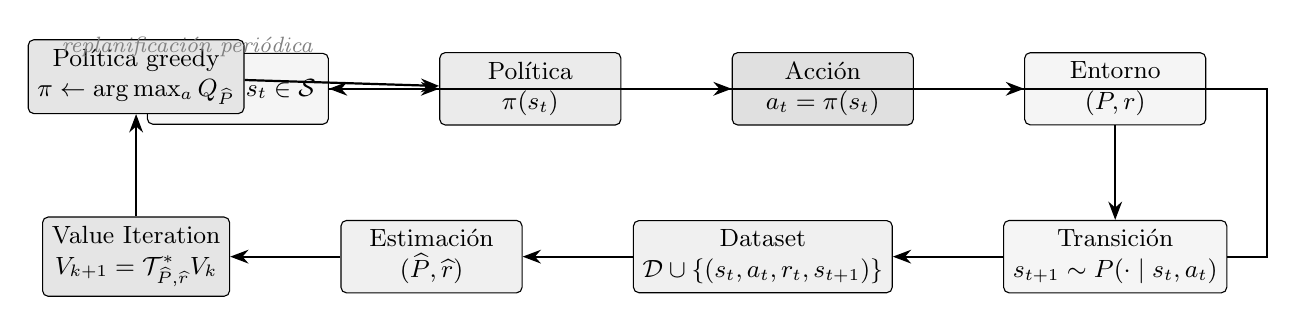
\begin{tikzpicture}[
  >=Stealth,
  node distance=1.3cm and 1.4cm,
  every node/.style={font=\small},
  block/.style={draw, rounded corners=2pt, align=center, minimum width=2.3cm, minimum height=0.9cm, fill=white},
  obs/.style={block, fill=gray!8},
  dec/.style={block, fill=gray!16},
  act/.style={block, fill=gray!24},
  est/.style={block, fill=gray!12},
  plan/.style={block, fill=gray!20},
  arr/.style={->, thick}
]
% Nodos
\node[obs] (state) {Estado $s_t\in\cS$};
\node[dec, right=of state] (policy) {Política\\ $\pi(s_t)$};
\node[act, right=of policy] (action) {Acción\\ $a_t=\pi(s_t)$};
\node[obs, right=of action] (env) {Entorno\\$(P,r)$};
\node[obs, below=1.2cm of env] (next) {Transición\\$s_{t+1}\sim P(\cdot\mid s_t,a_t)$};
\node[est, left=of next] (data) {Dataset\\$\mathcal{D}\cup\{(s_t,a_t,r_t,s_{t+1})\}$};
\node[est, left=of data] (estim) {Estimación\\$(\Phat,\rhat)$};
\node[plan, left=of estim] (vi) {Value Iteration\\$V_{k+1}=\cT^{*}_{\Phat,\rhat}V_k$};
\node[plan, above=of vi] (greedy) {Política greedy\\$\pi\leftarrow\arg\max_a Q_{\Phat}$};

% Flechas principales del ciclo
\draw[arr] (state) -- (policy);
\draw[arr] (policy) -- (action);
\draw[arr] (action) -- (env);
\draw[arr] (env) -- (next);
\draw[arr] (next) -- (data);
\draw[arr] (data) -- (estim);
\draw[arr] (estim) -- (vi);
\draw[arr] (vi) -- (greedy);
\draw[arr] (greedy) -- (policy);
% Feedback a estado
\draw[arr] (next.east) -- ++(0.5,0) |- (state.east);
% Etiqueta del ciclo
\node[font=\footnotesize\itshape, gray] at ($(vi)!0.5!(state)+(0,1.6)$) {replanificación periódica};
\end{tikzpicture}}
\caption{Pipeline del agente estadístico determinístico. El bloque
\emph{Value Iteration} es el único componente con garantía de
convergencia certificada; los bloques de \emph{Estimación} y
\emph{Dataset} heredan los sesgos de $\pibeh$ y de la representación de
estado. La flecha de retroalimentación cierra el ciclo entre transición
y siguiente estado.}
\label{fig:pipeline}
\end{figure}

El ciclo opera en dos escalas de tiempo distintas. En la escala corta
(paso a paso), el agente observa, decide con la política actual y
actualiza el dataset. En la escala larga (replanificación), reestima
$(\Phat,\rhat)$, itera Value Iteration hasta satisfacer el criterio de
parada $\norminf{V_{k+1}-V_k}<\varepsilon_{\mathrm{stop}}$ y recalcula
$\pi$ como política greedy respecto al último $V_k$.

La separación entre ambas escalas es un parámetro de diseño crítico:
replanificar en cada paso es caro y puede introducir inestabilidad;
replanificar muy rara vez conduce a políticas obsoletas si la
distribución de datos cambia. Una heurística razonable es replanificar
cuando el tamaño del dataset se ha duplicado o cuando un test de
estacionariedad sobre $\Phat$ detecta deriva significativa.

% =============================================================================
\section{Algoritmo determinista}
\label{sec:algoritmo}
% =============================================================================

\begin{theorem}[Value Iteration con modelo estimado]
\label{thm:vi-estimado}
Sea $\widehat{\cT}^{*}$ el operador de Bellman construido con
$(\Phat,\rhat)$. Bajo los supuestos de la Sección~\ref{sec:supuestos},
$\widehat{\cT}^{*}$ es una contracción de módulo $\gamma$ en
$\norminf{\cdot}$ y posee un único punto fijo
$\widehat{V}^{*}\in\R^{|\cS|}$. La sucesión
$V_{k+1}=\widehat{\cT}^{*}V_k$ converge geométricamente:
\[
  \norminf{V_k-\widehat{V}^{*}}
  \;\leq\;\frac{\gamma^k}{1-\gamma}\,\norminf{V_1-V_0}.
\]
\end{theorem}

\begin{proof}
La demostración es idéntica a la del operador verdadero $\cT^{*}$: el
argumento de contracción solo usa que $\Phat(\cdot\mid s,a)$ es una
distribución de probabilidad y que $\rhat$ está acotada, propiedades que
se heredan del estimador. El teorema de Banach--Caccioppoli se aplica
sin modificaciones.
\end{proof}

El subtítulo ``con modelo estimado'' es engañoso: el teorema garantiza
convergencia \emph{al punto fijo del modelo estimado}, no al punto fijo
verdadero. La distancia entre ambos es el verdadero objeto de interés y
no se controla con la cota a priori del Teorema~\ref{thm:vi-estimado}.

\subsection{Política greedy derivada}

Una vez que $V_k$ satisface el criterio de parada, se define la política
determinista
\[
  \pigreedy(s)
  \;\in\;\arg\max_{a\in\cA}\Bigl\{\rhat(s,a)
  +\gamma\sum_{s'}\Phat(s'\mid s,a)\,V_k(s')\Bigr\},
  \quad s\in\cS.
\]
Por el teorema de la política $\varepsilon$-óptima,
\[
  \norminf{V^{\pigreedy}-\widehat{V}^{*}}
  \;\leq\;\frac{2\gamma}{1-\gamma}\,\norminf{V_k-\widehat{V}^{*}},
\]
de modo que el error en valor se amplifica por un factor
$\dfrac{2\gamma}{1-\gamma}$ al traducirse en política. Para $\gamma=0.99$,
este factor es $198$: un error de valor de $0.01$ se convierte en un
error de política de hasta $1.98$, lo que destruye cualquier garantía
práctica si no se controla $\Delta_k$ con suficiente holgura.

\subsection{Criterio de parada recomendado}

Para garantizar un error de política (respecto al modelo estimado) menor
que $\varepsilon_{\pi}$, basta iterar hasta
\[
  \norminf{V_{k+1}-V_k}
  \;<\;\frac{(1-\gamma)^2\,\varepsilon_{\pi}}{4\gamma^2},
\]
que es la versión combinada del criterio a priori y del factor de
amplificación. Para $\gamma$ cercano a $1$, esto exige iteraciones del
orden de $(1-\gamma)^{-1}\log(1/\varepsilon_{\pi})$, lo que puede ser
computacionalmente prohibitivo pero es el precio formal de la garantía.

\subsection{Ejemplo numérico ilustrativo}

Considérese un MDP con dos estados $\cS=\{s_1,s_2\}$ y dos acciones
$\cA=\{a_1,a_2\}$, con $\gamma=0.9$, recompensas
$r(s_1,a_1)=1$, $r(s_1,a_2)=0$, $r(s_2,a_1)=r(s_2,a_2)=0$, y kernel
\[
  P(\cdot\mid s_1,a_1)=(0.5,0.5),\quad
  P(\cdot\mid s_1,a_2)=(1,0),
\]
\[
  P(\cdot\mid s_2,a_1)=(0.8,0.2),\quad
  P(\cdot\mid s_2,a_2)=(0,1).
\]
Tomando $V_0\equiv 0$, las primeras iteraciones de Value Iteration son
\[
  V_1=(1,0),\quad
  V_2=(1.45,0),\quad
  V_3=(1.6525,0),\quad
  V_4=(1.7436,0),
\]
y el punto fijo es $\Vopt=\bigl(\tfrac{1}{1-0.45},0\bigr)\approx(1.818,0)$.
El error decae geométricamente:
$\norminf{V_k-\Vopt}\leq\dfrac{0.9^k}{0.1}\norminf{V_1-V_0}=10\cdot 0.9^k$.
Para $\varepsilon=0.01$ se obtiene
$k_\varepsilon=\lceil\log(0.001)/\log(1/0.9)\rceil=66$ iteraciones.

Este ejemplo mínimo ilustra tres puntos. Primero, la convergencia es
efectivamente geométrica pero el prefactor $\norminf{V_1-V_0}/(1-\gamma)$
puede ser grande: aquí vale $10$, de modo que la cota a priori es muy
generosa respecto al error real. Segundo, la política greedy extraída de
$V_k$ coincide con $\pi^{*}$ desde $k=1$ en este caso sencillo, pero esto
\emph{no} es general: cuando dos acciones tienen valores cercanos, la
amplificación por $\dfrac{2\gamma}{1-\gamma}$ puede revertir el orden
durante varias iteraciones. Tercero, si reemplazamos el verdadero $P$ por
una estimación $\Phat$ con, digamos, $5\%$ de error en cada entrada, el
punto fijo se desplaza en una cantidad proporcional a
$\dfrac{\gamma}{(1-\gamma)^2}\norminf{\Phat-P}\approx 90\cdot 0.05\approx 4.5$
veces el error de estimación ---lo que ilustra concretamente la
sensibilidad espectral discutida en la Sección~\ref{sec:supuestos}.

% =============================================================================
\section{Modos de falla}
\label{sec:fallos}
% =============================================================================

El agente determinístico falla de cuatro maneras distintas, cada una
asociada a la rotura de un supuesto de la Sección~\ref{sec:supuestos}.
Identificar qué supuesto falló es esencial para diagnosticar al agente y,
sobre todo, para no atribuir a ``mala calibración de $\gamma$'' lo que en
realidad es un problema de diseño.

\subsection{Markov roto}

Si el espacio de estados es una proyección empobrecida del estado
verdadero ---típicamente porque se descartaron variables relevantes, se
agruparon estados heterogéneos o se acumuló ruido de medición--- la
propiedad de Markov falla. Síntomas: residuos de la ecuación de Bellman
correlacionados con el pasado, valor estimado que no coincide con el
valor empírico medio en trayectorias largas, política que se desempeña
mejor en simulación que en despliegue. La reparación no es estadística
sino de diseño: enriquecer $\cS$ con variables latentes o pasar a un
POMDP con creencias explícitas.

\subsection{$\Phat$ sesgado}

Si el dataset $\mathcal{D}$ proviene de una política $\pibeh$
diferente de la política objetivo, la estimación $\Phat$ y $\rhat$
heredan el sesgo de muestreo. Esto no es un defecto del estimador, es
un defecto del diseño experimental: la información disponible no es
representativa del régimen operativo. Síntomas: divergencia entre el
valor predicho $\widehat{V}^{*}$ y el valor observado empíricamente en
despliegue, alta varianza en estados poco visitados por $\pibeh$.
Reparación: importance sampling, modelos causales, o recolección
on-policy adicional.

\subsection{Ausencia de overlap}

Si existe $(s,a)$ tal que $\pibeh(a\mid s)=0$ pero $\pi(a\mid s)>0$,
no hay información para estimar $Q(s,a)$ en ese par. El agente
determinístico puede declarar $\pi(s)=a$ como óptima sobre la base de
ruido numérico en $\Phat$, sin posibilidad de validación. Síntomas:
acciones óptimas en estados con cero visitas de $\pibeh$, intervalos de
confianza bootstrap infinitos para $V^{\pi}$, comportamiento errático al
desplegar. Reparación: restringir $\pi$ al soporte de $\pibeh$, o
realizar exploración dirigida (epsilon-greedy sobre $\pibeh$) antes de
replanificar.

\subsection{Explotación prematura}

La ausencia de exploración estocástica (como Thompson Sampling o UCB en
el caso de bandidos) expone al agente a explotar una política que parece
óptima bajo datos limitados pero que no lo es en el régimen verdadero.
Síntomas: política que colapsa a una sola acción para la mayoría de los
estados, valor empírico que decrece con el tiempo a pesar de converger
$\norminf{V_{k+1}-V_k}$, error sistemático en subpoblaciones no
representadas. Reparación: añadir una capa exploratoria ---$\varepsilon$-greedy,
muestreo de Thompson sobre $\Phat$, o UCB sobre $\Vpi$--- y conservar la
política determinística solo para inferencia y análisis.

\subsection{Ilustración clínica: escenario SSCH}

En el escenario clínico del SSCH (Síndrome Subclínico de Cuidados
Hipertensivos, mencionado en el material de partida), los estados
codifican niveles de severidad y comorbilidades del paciente, y las
acciones corresponden a distintas clases de antihipertensivos: IECA,
ARA-II, bloqueadores cálcicos, diuréticos. Supóngase que en el estado
$s_3$ (hipertensión moderada con daño renal incipiente), Value Iteration
sobre el modelo estimado $\Phat$ indica que la acción óptima es
$\pi^{*}(s_3)=\text{IECA}$.

La determinidad de $\pi^{*}$ implica que \emph{todo} paciente que llegue a
$s_3$ recibirá IECA. Si la política de comportamiento $\pibeh$ que generó
$\mathcal{D}$ rara vez recetó ARA-II en $s_3$, el estimador
$\Phat(s'\mid s_3,\text{ARA-II})$ tiene alta varianza y, posiblemente, un
sesgo sistemático. El agente, sin embargo, lo trata como un parámetro
cierto y declara IECA como óptimo. En pacientes atípicos ---por ejemplo,
aquellos con tos seca persistente como efecto adverso a IECA, una
variable latente no incluida en $\cS$--- la acción ARA-II habría sido
superior, pero el agente no puede siquiera detectarlo: el dato no existe
en $\mathcal{D}$ y la política no explora. La contracción del operador de
Bellman garantiza convergencia \emph{al punto fijo del modelo}, no al
óptimo clínico real. Esta brecha, silenciosa en simulación, se manifiesta
como deterioro renal acelerado en un subgrupo no representado durante el
despliegue.

\begin{remark}[La determinidad es un punto ciego]
\label{rem:determinidad}
La ausencia de aleatoriedad en la política no es una virtud: es una
renuncia a recoger información. En el isomorfismo Wald--MDP, el caso
$k=1$ (un solo brazo) corresponde a los bandidos, y ahí la teoría
(Thompson, UCB, KL-UCB) muestra que la exploración es \emph{necesaria}
para alcanzar optimalidad regret. El agente determinístico del
Capítulo~8 elimina la exploración al asumir que el modelo es conocido;
cuando este supuesto cae, la determinidad deja de ser óptima y pasa a
ser una limitación estructural.
\end{remark}

% =============================================================================
\section{Conexión con el Capítulo 11 y con el isomorfismo Wald--MDP}
\label{sec:conexion}
% =============================================================================

\subsection{Mezcla lenta, intervalos de confianza anchos}

Cuando $\gamma\to 1$, el tiempo de mezcla efectivo
$\tau_{\mathrm{mix}}$ de la cadena inducida por $\pi^{*}$ crece como
$(1-\gamma)^{-1}$. Esto afecta directamente a la inferencia estadística
sobre el valor: la varianza asintótica del estimador de Monte Carlo del
retorno descontado satisface
\[
  \sigma^2
  \;\propto\;\tau_{\mathrm{mix}}\cdot\mathrm{Var}(r)
  \;\sim\;\frac{\mathrm{Var}(r)}{1-\gamma},
\]
y los intervalos de confianza ---ya sean por bootstrap o por CLT para
cadenas de Markov--- crecen como $(1-\gamma)^{-1/2}$. El mismo factor
espectral que dificulta la convergencia de Value Iteration dificulta
también la inferencia sobre el valor. Planificación e inferencia no son
dos problemas separados: comparten raíz espectral.

\subsection{Isomorfismo Wald--MDP}

La regla de decisión de Wald $\delta:\mathcal{X}\to\cA$ minimiza el
riesgo $\risk(\theta,\delta)=\mathbb{E}_{\theta}\bigl[L(\theta,\delta(X))\bigr]$
en un problema estático de un solo paso. La política $\pi:\cS\to\cA$ del
MDP extiende esta idea al caso secuencial: minimiza un riesgo
\emph{recursivo} donde la decisión actual condiciona el estado futuro y,
con él, las decisiones posteriores. La correspondencia formal es
\[
  \risk^{*}(\theta,\delta)\;\longleftrightarrow\;-V^{*}(s),
\]
donde $V^{*}$ es la función de valor óptima y $\theta$ es el parámetro
del modelo. Bajo este isomorfismo, el agente estadístico determinístico
del Capítulo~8 es la encarnación recursiva de una regla $\delta$
estática, pero sin la robustez minimax que Wald desarrolló para el caso
estático. Cuando la identificación del modelo falla (Markov roto,
$\Phat$ sesgado, no-overlap), el agente pierde toda garantía y la
política óptima computada se convierte en una ilusión de control.

% =============================================================================
\section{Recomendaciones de diseño}
\label{sec:recomendaciones}
% =============================================================================

A partir del análisis anterior, la construcción de un agente
determinístico robusto requiere un protocolo de diseño explícito. Las
siguientes recomendaciones no son opcionales: cada una responde a un
modo de falla identificado en la Sección~\ref{sec:fallos}.

\begin{enumerate}[label=\textbf{R\arabic*.}, leftmargin=2.5em, noitemsep]
  \item \textbf{Auditar la suficiencia de $\cS$ antes de iterar.}
        Realizar tests de Markov sobre residuos de Bellman: si
        $\Vpi(s_t)-\bigl[r(s_t,a_t)+\gamma\,\Vpi(s_{t+1})\bigr]$ está
        correlacionado con observaciones pasadas, el estado no es
        suficiente y la arquitectura debe revisarse antes de cualquier
        optimización.

  \item \textbf{Reportar intervalos de confianza para $\widehat{V}^{*}$.}
        La cota $\dfrac{\gamma^k}{1-\gamma}\norminf{V_1-V_0}$ controla el
        error numérico, no el error estadístico. Es indispensable
        acompañar $\widehat{V}^{*}$ con bandas bootstrap o CLT para
        cadenas, especialmente cuando $\gamma$ es cercano a $1$.

  \item \textbf{Verificar overlap explícitamente.}
        Antes de desplegar $\pi$, calcular
        $\sum_{s,a}\pi(a\mid s)\,\mathbb{1}\{\pibeh(a\mid s)=0\}$: si es
        positivo, existen pares no identificables y la política no es
        validable. En tal caso, restringir $\pi$ al soporte de $\pibeh$ o
        realizar exploración dirigida.

  \item \textbf{Calibrar $\gamma$ con el horizonte efectivo.}
        Elegir $\gamma$ de modo que
        $H_{\mathrm{eff}}=(1-\gamma)^{-1}$ sea coherente con el horizonte
        operativo del problema. $\gamma=0.99$ implica $H_{\mathrm{eff}}=100$:
        si las trayectorias disponibles son de longitud $20$, el agente
        está extrapolando masivamente.

  \item \textbf{Añadir una capa exploratoria para despliegue.}
        La política determinística es adecuada para análisis e inferencia
        off-policy, pero no para despliegue ciego. Combinar $\pi$ con
        $\varepsilon$-greedy o Thompson sobre $\Phat$ preserva la
        interpretabilidad del agente principal mientras recopila
        información para futuras replanificaciones.

  \item \textbf{Replanificar con trigger estadístico, no cronológico.}
        En lugar de replanificar cada $N$ pasos, hacerlo cuando un test
        de deriva sobre $\Phat$ lo indique, o cuando el tamaño del
        dataset se duplique. Esto evita tanto la obsolescencia de la
        política como la inestabilidad por replanificación excesiva.
\end{enumerate}

% =============================================================================
% Resumen
% =============================================================================

\bigskip
\noindent\rule{\textwidth}{0.4pt}

\smallskip
\noindent\textbf{Síntesis.}

{\sloppy
El agente estadístico determinístico es una máquina elegante de
recursión de riesgo, pero su poder descansa sobre presupuestos
espectrales: suficiencia del estado, conocimiento o estimación perfecta
de $P$, estacionariedad y overlap. Cuando estos se rompen ---y en la
mayoría de aplicaciones inteligentes se rompen--- la política óptima
computada se convierte en una ilusión de control. Quien ignora este
punto no construye un agente inteligente; construye un optimizador
frágil que colapsa bajo la complejidad del mundo real. La optimalidad es
siempre condicional al modelo, y el modelo siempre miente, aunque sea
un poco.
}

\noindent\rule{\textwidth}{0.4pt}

\end{document}
% =============================================================================
% FIN DEL DOCUMENTO
% =============================================================================
